\documentclass[sigplan, screen]{acmart}
\usepackage[german]{babel}
\usepackage{fancyhdr}
\usepackage{listings}

\AtBeginDocument{%
  \providecommand\BibTeX{{%
    \normalfont B\kern-0.5em{\scshape i\kern-0.25em b}\kern-0.8em\TeX}}}

\definecolor{backcolour}{rgb}{0.95,0.95,0.92}
\definecolor{lightgray}{rgb}{.9,.9,.9}
\definecolor{darkgray}{rgb}{.4,.4,.4}
\definecolor{purple}{rgb}{0.65, 0.12, 0.82}
\definecolor{lightgreen}{rgb}{0.45, 0.8, 0.45}

\lstdefinelanguage{JavaScript}{
  keywords={break, case, catch, continue, debugger, default, delete, do, else, false, finally, for, function, if, in, instanceof, new, null, return, switch, this, throw, true, try, typeof, var, void, while, with},
  keywordstyle=\color{purple}\bfseries,
  ndkeywords={type, class, export, boolean, throw, implements, import, this},
  ndkeywordstyle=\color{darkgray}\bfseries,
  identifierstyle=\color{black},
  sensitive=false,
  comment=[l]{//},
  morecomment=[s]{/*}{*/},
  commentstyle=\color{gray}\ttfamily,
  stringstyle=\color{lightgreen}\ttfamily,
  morestring=[b]',
  morestring=[b]"
}

\lstdefinestyle{mystyle}{
  language=JavaScript,
  basicstyle=\ttfamily\footnotesize,
  breakatwhitespace=false,         
  breaklines=true,                     
  keepspaces=true,                 
  numbers=left,                    
  numbersep=5pt,                  
  showspaces=false,                
  showstringspaces=false,
  showtabs=false,                  
  tabsize=2
}

\lstset{style=mystyle}

\setcopyright{none}
\settopmatter{printacmref=false}
\renewcommand\footnotetextcopyrightpermission[1]{}
\copyrightyear{2022}
\acmYear{2022}

\acmBooktitle{Hauptseminar II WiSe 22/23, gehalten von Kevin Linne, M.Sc.}

\begin{document}

\title{Möglichkeiten zur asynchronen Kommunikation zwischen Webbrowser und Server}

\author{Hendrik Wagner}
\email{hendrik.wagner@mni.thm.de}

\affiliation{%
  \institution{Technische Hochschule Mittelhessen}
  \streetaddress{Wiesenstraße 14}
  \city{Gießen}
  \state{Hessen}
  \postcode{35390}
  \country{Germany}
}

\begin{abstract}
  Die Kommunikation zwischen Webbrowser und Server wird klassischerweise durch den Client (in der Regel ein Webbrowser) initiiert.
  Dieser fragt den Inhalt einer Website an, und kann später weitere Inhalte laden oder Daten übermitteln.
  Der Server kann aber keine Daten nachträglich an den Client senden, wenn dieser diese nicht aktiv anfragt.
  In diesem Artikel werden verschiedene Möglichkeiten zur fortlaufenden Kommunikation zwischen Client und Server vorgestellt und analysiert.
  Dabei werden die Vor- und Nachteile der einzelnen Methoden aufgezeigt.
\end{abstract}

\keywords{web, http, WebSockets, polling, bidirectional communication, asynchronous communication}

\maketitle
\lhead{\small Möglichkeiten zur asynchronen Kommunikation zwischen Webbrowser und Server}
\rhead{\small Hendrik Wagner}

\tableofcontents
\newpage

% Möglichkeiten für Client-Server Kommunikation nach Aufruf einer Website
% Auseinandersetzung mit...
% - Was sind und wie funktionieren Websockets (Spezifikation), Polling, Long Polling
% - Realisierungen (insb. Serverside-Setup von Websockets, ggf. Polling-Algorithmen) 
% - Vergleich von manuell implementierten Websockets, Polling (Auch mit Blick auf Performance, TCP packets)
% - Vergleich/Analyse von existierenden Websocket-Frameworks

% - statistiken (verbreitung, wie wirds eingesetzt)
% - umsetzung von ws durch aktuelle frameworks, was machen die, welche frameworks gibt es
% - spezifikation von ws

\section{Einleitung}

Gilt es, eine Website mit bidirektionaler bzw. asynchroner Kommunikation (z. B. vom Server bereitgestellten Aktualisierungen) zu realisieren,
so muss eine Auswahl zwischen verschiedenen Ansätzen gewählt werden.
Ein solcher Fall kann eine Chatanwendung sein, in welcher der Server von einem Client erhaltene Nachrichten an andere Clients weitersendet.
Ein weiteres Beispiel wäre eine rechenintensive Anwendung,
in der eine Berechnung nach einiger Zeit erfolgt und der Server das Ergebnis an den Client melden soll.
Da der Server unter HTTP nicht ohne weiteres eine Nachricht an einen Client senden kann, muss dieser die Nachricht anfordern --
diese simple Art des Nachrichtenempfangs nennt man \emph{Polling}, also die wiederholte Abfrage nach neuen Nachrichten.
Neben diesem Ansatz gibt es \emph{WebSockets}, welche eine TCP/UDP-ähnliche Kommunikation im Web ermöglichen.

\section{Vorstellung der Kommunikationsvarianten}

Zunächst werden die Kommunikationsvarianten in ihrer Funktionsweise erklärt und vorgestellt.
In späteren Kapiteln wird ebenfalls auf deren Implementierung sowie auf Frameworks eingegangen.

\subsection{Klassisches Polling}

Unter dem 1990 eingeführten \cite[Abs. 1.2]{fielding_http_2022} HTTP-Protokoll gibt es eine Reihe von Anfragen, die der Client an den Server senden kann \cite{noauthor_http_nodate}.
Das Protokoll definiert dabei explizit einen Client (in unserem Fall der Browser), welcher Anfragen an den Server (Bereitstellender der Webinhalte) versendet.
Dieser wartet auf Anfragen und beantwortet diese \cite[Abs. 1.3]{fielding_http_2022}.

Für das Vorhaben sind GET-Requests besonders relevant, also klassische Abfragen von Inhalten mittels HTTP.
Polling, in diesem Anwendungsfall wohl am besten übersetzt mit \emph{zyklische Absuche} oder \emph{Sendeaufruf},
beschreibt in der Webentwicklung das regelmäßige Abrufen (in einem Intervall $\Delta$) von neuen Inhalten.
Gibt es Nachrichten, die der Server bereitstellen möchte, beantwortet dieser die Anfrage mit den neuen Inhalten --
andernfalls wird der Antwortkörper leer sein.

\begin{figure}[H]
  \centering
  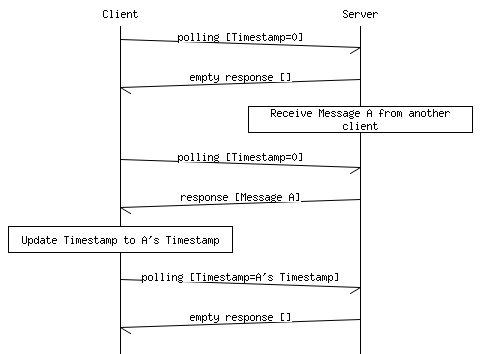
\includegraphics[width=.45\textwidth]{assets/msc/polling.png}
  \caption[Nachrichtenempfang bei Polling-Kommunikation]{Beispiel von Nachrichtenempfang bei einer klassischen Polling-Kommunikation.
    Der Client sendet regelmäßig eine Anfrage an den Server, welche entweder mit leerer Antwort oder mit neuen Inhalten beantwortet wird.}
  \label{fig:polling}
\end{figure}

\begin{figure}[H]
  \centering
  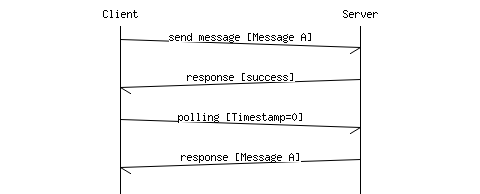
\includegraphics[width=.45\textwidth]{assets/msc/polling-send.png}
  \caption[Nachrichtenversand bei Polling-Kommunikation]{Beispiel von Nachrichtenversand bei einer klassischen Polling-Kommunikation.
    Der Client sendet eine Nachricht an den Server, welche daraufhin mittels polling abgerufen werden kann.}
    \label{fig:polling_send}
\end{figure}

Das Hauptproblem mit Polling ist der entstehende Header Overhead, der für den gesamten Zeitraum in den regelmäßigen Abfragen besteht.
Dadurch entsteht eine Netzwerkbelastung, welche keine tatsächlichen Informationen übermittelt.
In der in späteren Abschnitten vorgestellten Chatanwendung handelt es sich so zum Beispiel um 156 Bytes, die sekündlich vom Server übermittelt werden,
aber lediglich ein leeres JSON-Array enthalten.


\subsubsection{Spezifikation}

Polling ist in der Spezifikation von HTTP nicht definiert, es handelt sich hierbei um eine Implementierung des Clients und des Servers.
Meist wird Polling durch JavaScript-Code realisiert, welcher in einem bestimmten Intervall (z. B. alle 5 Sekunden) eine Anfrage an den Server sendet.
Diese Anfrage ist ein GET-Request, welcher die URL der Anwendung enthält.
Wie der Server auf diese Anfrage antwortet, ist Implementierungsabhängig:
So könnte er zum Beispiel den gesamten abgefragten Inhalt bei jeder Anfrage übermitteln, oder nur Änderungen, die dieser Client noch nicht übermittelt bekommen hat.
Eine solche Optimierung setzt allerdings voraus, dass der Server in der Lage ist, zu identifizieren, welche Änderungen der Client bereits erhalten hat.

\subsection{Long Polling}

Eine Optimierung des Polling-Konzepts ist das sog. \emph{Long Polling}.
Dabei wird die Antwort auf eine HTTP-Anfrage zurückgehalten, bis der Server eine Nachricht versenden will \cite{noauthor_long_2021}.

\begin{figure}[H]
  \centering
  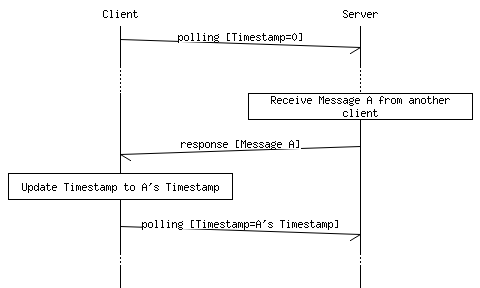
\includegraphics[width=.45\textwidth]{assets/msc/long-polling.png}
  \caption[Nachrichtenempfang bei Long Polling]{Beispiel von Nachrichtenempfang bei Long Polling.
  Der Server beantwortet die Anfrage des Clients erst, wenn er eine Nachricht hat, die er übermitteln möchte.
  Der Nachrichtenversand verläuft analog zu Polling.}
  \label{fig:long_polling}
\end{figure}

Probleme von Long Polling sind unter anderem der (im Vergleich zu klassischem Polling reduzierter, aber weiterhin präsenter)
Header Overhead, mögliche Timeouts und Ressourcen, die in Vorbereitung auf eine eingehende Nachricht vom Betriebssystem
zu Verfügung gestellt werden. \cite[Abs. 2.2]{saint-andre_known_2011}.

\subsection{Streaming}

Eine weitere Optimierung des Polling-Konzepts ist das sog. \emph{Streaming},
welches die HTTP Transferkodierung Chunking (vgl. \cite[Abs. 7.1]{fielding_http_2022}) verwendet,
also dem Aufspalten der Antwort in mehrere Packets, in welchen dann einzelne Nachrichten versendet werden.
So kann die Anzahl an Anfragen ausgehend vom Client an den Server auf eine reduziert werden --
der Server terminiert nie die Antwort auf die erste Anfrage \cite[Abs. 3]{saint-andre_known_2011}.

\begin{figure}[H]
  \centering
  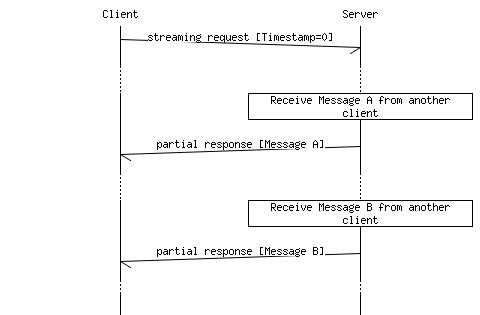
\includegraphics[width=.45\textwidth]{assets/msc/streaming.png}
  \caption[Nachrichtenempfang bei Streaming]{Beispiel von Nachrichtenempfang bei Streaming.
  Der Client initiiert den Streaming-Prozess durch eine einmalige Anfrage.
  Daraufhin sendet der Server Teilantworten an den Client, sobald neue Nachrichten verfügbar sind.
  Der Nachrichtenversand verläuft analog zu Polling.}
  \label{fig:streaming}
\end{figure}

Mit Streaming werden einige Nachteile von Polling beglichen, andere -- insb. mögliche Timeouts und unnötig reservierte Ressourcen -- bleiben bestehen.
Zusätzlich besteht das Risiko, dass diese Form von Kommunikation nicht auf allen Systemen funktioniert --
Proxys können Pakete bündeln und erst verzögert weiterleiten, wodurch Pakete ggf. nicht zeitgetreu, gebündelt oder aufgespalten ankommen \cite[Abs. 3.2]{saint-andre_known_2011}.

\subsection{WebSockets}

WebSockets sind ein vom IETF\footnote{Internet Engineering Task Force.} entwickeltes Protokoll,
welches 2011 als Standard veröffentlicht wurde \cite{melnikov_websocket_2011}.
Grund für dessen Entstehung ist unter anderem die Erkenntnis, dass der Versuch HTTP zu verwenden,
um bidirektionale Kommunikation zu ermöglichen, vermeidbare Komplexität und Ineffizienz mit sich bringt \cite[S. 137f]{lubbers_pro_2010}.
Es ist anzumerken, dass die vorgestellten Polling-Varianten das HTTP-Protokoll effektiv missbrauchen,
um serverseitige Kommunikation zu ermöglichen:

\begin{itemize}
  \item Polling beinhaltet das Versenden von redundanten Anfragen, welche ohne Inhalt beantwortet werden,
  \item Long Polling simuliert eine Verbindung mit (sehr) hoher Latenz um eine Antwort herauszuzögern und
  \item Streaming verwendet HTTP Chunking, um innerhalb einer Response alleinstehende Nachrichten zu senden.
\end{itemize}

Diesen Missbrauch haben WebSockets nicht -- es handelt sich hierbei um ein komplett neues Protokoll,
welches diese Problemstellung direkt adressiert (vgl. \cite[Abs. 1.1]{melnikov_websocket_2011}),
indem es eine TCP-Verbindung zwischen Client und Server aufbaut und unterstützt.
Genauer baut WebSockets einen Tunnel zwischen TCP und IP auf, sodass darauffolgend TCP-Kommunikation Systemübergreifend erfolgen kann (vgl. \cite[Abs. 1.5]{melnikov_websocket_2011}).
HTTP wird dann lediglich für die initialen Handshakes verwendet -- danach nicht mehr.


\begin{figure}[H]
  \centering
  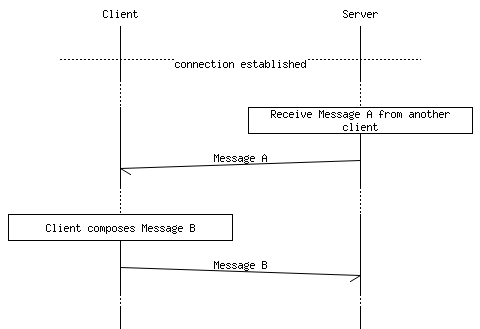
\includegraphics[width=.45\textwidth]{assets/msc/websockets.png}
  \caption[Nachrichtenaustausch bei WebSockets]{Beispiel von Nachrichtenaustausch bei WebSockets.
  Nach dem Handshake wird eine TCP-Verbindung zwischen Client und Server aufgebaut.
  Von nun an können Nachrichten in beide Richtungen ausgetauscht werden.}
  \label{fig:websockets}
\end{figure}

\subsubsection{Spezifikation}
Um eine Verbindung über einen WebSocker aufzubauen, wird zunächst vom Client aus eine HTTP-Anfrage gesendet.
Gemäß der Spezifikation muss es sich hierbei um eine GET-Request an den Pfad, auf dem der WebSocket hinterlegt ist, handeln.

Wäre die WebSocket URI \texttt{ws://example.org/chat}, so wäre die erste Zeile der HTTP-Anfrage \texttt{GET /chat HTTP/1.1} \cite[Abs. 4.1]{melnikov_websocket_2011}.
Zusätzlich müssen in der Anfrage unter anderem der Host (hier \texttt{Host: example.org}) und die Intention (Felder \texttt{Connection: Upgrade} und \texttt{Upgrade: websocket}) als Headerfelder übermittelt werden.

Der Server antwortet auf diese Anfrage mit einer HTTP-Response, welche entweder den Statuscode 101 \emph{Switching Protocols} oder einen Fehlercode enthält.
Zudem meldet er bei erfolgreichem Protokollwechsel die vom Client angegebene Intention zurück.

Wurde die Verbindung vom Server akzeptiert, können nun Client und Server direkt miteinander kommunizieren.
Für die Datenübermittlung sieht das WebSocket Protokoll eine auch in anderen Protokollen ähnlich vertretenes Frame-System vor,
also dem Versenden von Daten in Form von Frames, welche jeweils einen Header und eine Payload enthalten.
Header enthalten u. A. den Opcode\footnote{Opcodes (\emph{Operation Codes}, dt. \emph{Befehlscode}) können bei WebSockets Frames mit Text- oder Binärdaten ankündigen, eine vorherige Frame fortsetzen, die Verbindung schließen, oder einen Ping/Pong markieren.} und die Payload-Länge (vgl. \cite[Abs. 5.2]{melnikov_websocket_2011}).


\section{Beispielhafte Implementierungen}

Um die Unterschiede zwischen den Kommunikationsvarianten ersichtlich zu machen, werden diese für eine Chat-Applikation implementiert.
Dabei wird jeweils auf die Client- und Serverseitige Implementierung eingegangen.

Die Realisierung erfolgt in TypeScript, wobei die Serverseitige Implementierung auf Node.js basiert.
Der Client benutzt das Vue.js-Framework mit Vuetify, um die Darstellung zu vereinfachen.
Implementierungen in anderen Frameworks erfolgen analog.


\subsection{Implementierung von Polling}

Für die Implementierung von Polling verwaltet der Server eine Liste der letzten 100 Nachrichten.
Neue von einem Client übermittelte Nachrichten werden mit Autor, Zeitstempel und Text in diese Liste eingefügt.
Fragt ein Client die Liste ab, so erhält er die letzten 100 Nachrichten zurück.
Der Client übermittelt dabei den Zeitstempel der letzten Nachricht, die er erhalten hat.
So kann der Server nur die Nachrichten zurückgeben, die nach diesem Zeitstempel eingegangen sind.

Es wird nicht auf die Darstellung der Nachrichten oder des Chats eingegangen, da dies nicht relevant für die Implementierung ist.
Entsprechende Codeabschnitte sind daher ausgelassen.
Die vollständige Implementierung ist im Repository \cite[\texttt{code/client/src/components/PollingChat.vue}]{wagner_seminar2022_2022} zu finden.


\begin{lstlisting}[caption={Beispielhafte Nachricht}, label={lst:polling-json}, numbers=none]
{
  content: "Hello World!",
  sender: "Alice",
  timestamp: "2022-12-04T19:29:13.455Z"
}
\end{lstlisting}

\subsubsection{Polling Server}



\subsubsection{Polling Client}

Der Client besteht aus der Komponente \texttt{PollingChat.vue}, welche die Funktionen zum Senden und Empfangen von Nachrichten enthält.
Die Darstellung, sowie die Speicherung von Nachrichten und Nutzdaten erfolgt in der Komponente \texttt{ChatPage.vue} (vgl. jeweils \cite[\texttt{code/client/src/components/}]{wagner_seminar2022_2022}).

\begin{lstlisting}[caption={Polling Client: Nachricht senden}, label={lst:polling-server-send-message}, firstnumber=18]
const sendMessage = async (msg: Message) => {
  await fetch("http://localhost:8082/polling/send", {
    method: "POST",
    headers: {
      "Content-Type": "application/json",
    },
    body: JSON.stringify(msg),
  });
};
\end{lstlisting}

Um eine Nachricht zu versenden, wird lediglich eine HTTP POST-Anfrage an die URL \texttt{/polling/send} gesendet.
Die Nachricht wird dabei als JSON-Objekt in der Anfrage übermittelt.

\begin{lstlisting}[caption={Polling Client: Nachrichten abfragen}, label={lst:polling-server-get-messages}, firstnumber=29]
const fetchMessages = async () => {
  const nextTimestamp = new Date().toISOString();
  const response = await fetch("http://localhost:8082/polling", {
    method: "POST",
    headers: {
      "Content-Type": "application/json",
    },
    body: lastMessageTimestamp,
  });
  if (response.ok) {
    if (httpError.value) {
      httpError.value = false;
    }
    
    emit("appendMessages", await response.json());
    lastMessageTimestamp = nextTimestamp;
  } else {
    httpError.value = true;
    httpErrorMessage.value = await response.text();
  }
};

const interval = setInterval(fetchMessages, 2000);
\end{lstlisting}

Mittels einer HTTP POST-Anfrage an die URL \texttt{/polling} werden die Nachrichten abgefragt.
Die Anfrage enthält dabei den Zeitstempel der letzten Nachricht, die der Client erhalten hat, als string.
Der Server antwortet mit einer Liste von Nachrichten, die nach diesem Zeitstempel eingegangen sind.
Diese werden anschließend an die Komponente \texttt{ChatPage.vue} mittels des Events \texttt{appendMessages} übermittelt.

Um die Nachrichten regelmäßig abzufragen, wird ein Interval gesetzt, welches alle zwei Sekunden die Funktion \texttt{fetchMessages} aufruft.
Dieses Interval wird bei der Initialisierung der Komponente gesetzt und bei der Entfernung der Komponente wieder gelöscht.



\subsection{Implementierung von Long Polling}

\dots

\subsection{Implementierung von WebSockets}

\subsubsection{WebSocket Client}

\subsubsection{WebSocket Server}

\section{Vergleiche zwischen Kommunikationsvarianten}


\subsection{Analyse der Implementierungen}

Vor- und Nachteile
Performance?

… Die Latenzen überschneiden sich mit Messungen getätigt im Rahmen eines Papers von Pimentel und Nickerson \cite{pimentel_communicating_2012}.

\subsection{Generelle Feststellungen}

Notabel ist auch die Reduktion in Overhead, welcher bei klassischem Polling durch HTTP-Header entsteht.
Üblicherweise sind HTTP-Header zwischen 200 und 2.000 Bytes groß \cite{noauthor_spdy_nodate}.
Dies kann einen ernsthaften Effekt auf die Netzwerkbelastung haben, besonders wenn die Polling- oder Nachrichtenfrequenz hoch ist.
So würden 1.000 Nutzer, die sekündlich Nachrichten anfragen, allein durch die Header etwa 6 Mbps an Netzwerkdurchsatz verursachen \cite{lubbers_html5_nodate}.
Dieser Netzwerkdurchsatz entfällt durch Websockets.

\section{Vorstellung von Frameworks}

Es gibt Frameworks, die das Implementieren von asynchroner Kommunikation erleichtern.

\subsection{Socket.IO}

Was ist das? Wie ist es besser oder schlechter für die Implementierung als Chat-App? Performance?

\subsection{Faye}

\section{Fazit}


\bibliographystyle{literature/bibtex/IEEEtran}
\bibliography{literature/literature}

\listoffigures

\end{document}
\endinput
%%
%% End of file `sample-sigplan.tex'.
